\subsection{Tous ensemble}

Toutes les équipes dans l'entreprise travaillent en suivant la méthodologie Agile, et chaque équipe choisit l'implémentation qui lui convient le mieux.

D'une façon globale, Bonitasoft travaille avec le framework représenté dans la Figure \ref{frame_safe}

\begin{figure}[!ht]
\centering
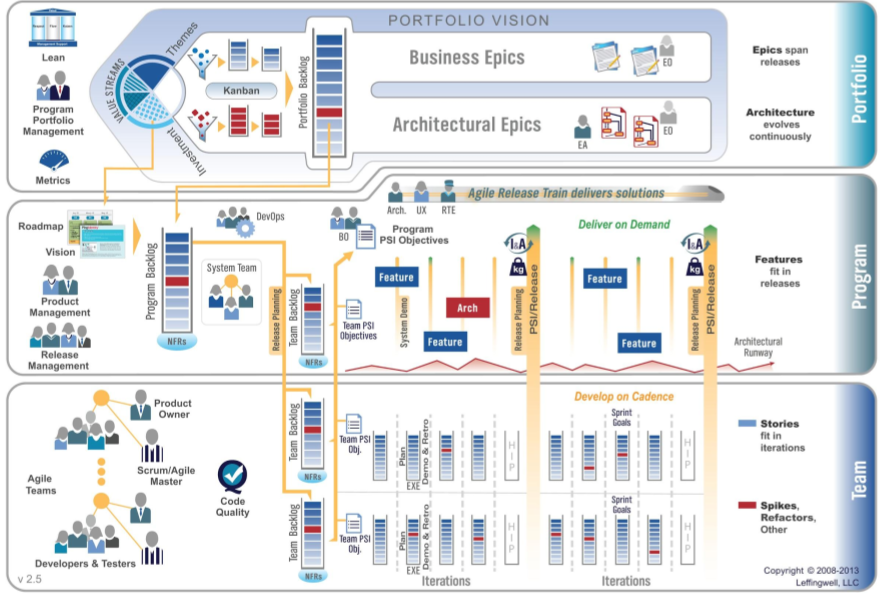
\includegraphics[width=\textwidth,keepaspectratio]{safe_framework.png}
\caption{Cadre de Travail \cite{safe}}
\label{frame_safe}
\end{figure}

Nous voyons dans la partie supérieure que la vision, les fonctionnalités et l'architecture de haut niveau sont définis dans le Comité Produit et le CEO.

Au milieu, le portfolio est traité et organisé par le Product Manager.

Finalement, il est développé par l'équipe de développeurs avec un \enquote{Product Owner} et le \enquote{Scrum Master} qui dirige.

Dans la Figure \ref{fig:example_epic}, nous voyons un exemple des \enquote{Epics} avec les \enquote{Issues} liés.
\begin{figure}[!ht]
\centering
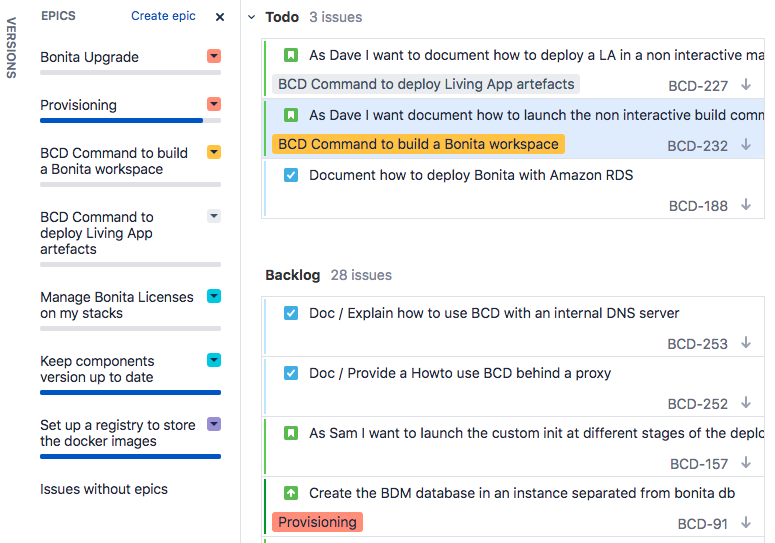
\includegraphics[width=\textwidth,keepaspectratio]{jira_epics_bl.png}
\caption{Exemple de Epics JIRA BCD}
\label{fig:example_epic}
\end{figure}
